\section{Wheel Shaft Assembly}\label{sec:wheel_shaft_assembly}
The wheel shaft assembly consists of a combination of parts such as bearings, seals and structural members. The assembly needed to be compact, cost efficient and easy to assemble with manufacturability in mind. %With the shaft being the main supporting component connecting the wheels to the drive box, much strength analysis has been conducted for it with varied materials and profiles. The rim mount which boasts the wheel onto the shaft also needed to be an elegant solution that provided self centering fastening. Taper roller bearings were also needed to handle the large axial forces induced by the skid steer motions. In order to house the bearings close to the drivebox, a bearing housing was designed in such a way that limits the flex in the shaft. To run a dry drivebox, radial seals were added to either side of the bearings to contain the grease, but also help limit contamination from the outside environment.

\begin{figure}[h]\centering
	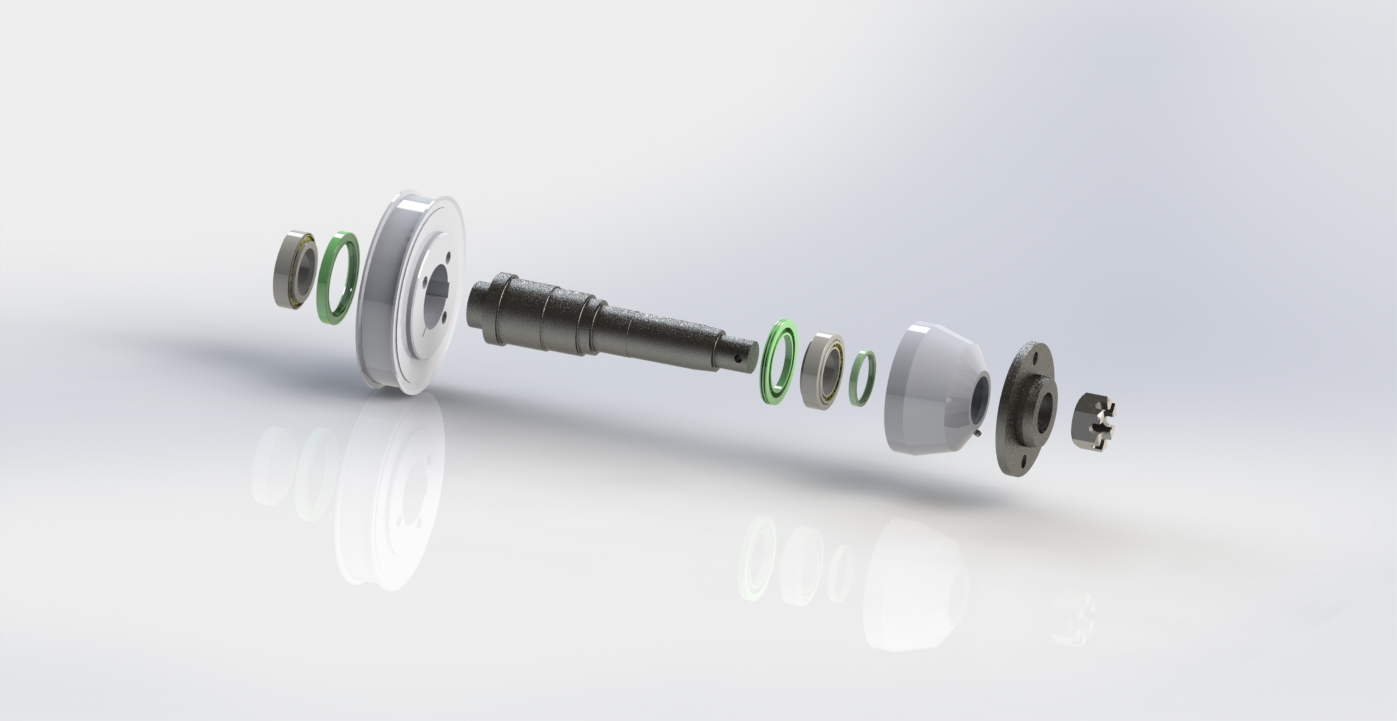
\includegraphics[width=.7\linewidth]{images/explode_wheel_assembly.jpg}
	\caption{Exploded view of wheel shaft assembly.}
	\label{fig:wheel_explode}
\end{figure}

\begin{figure}[h]\centering
	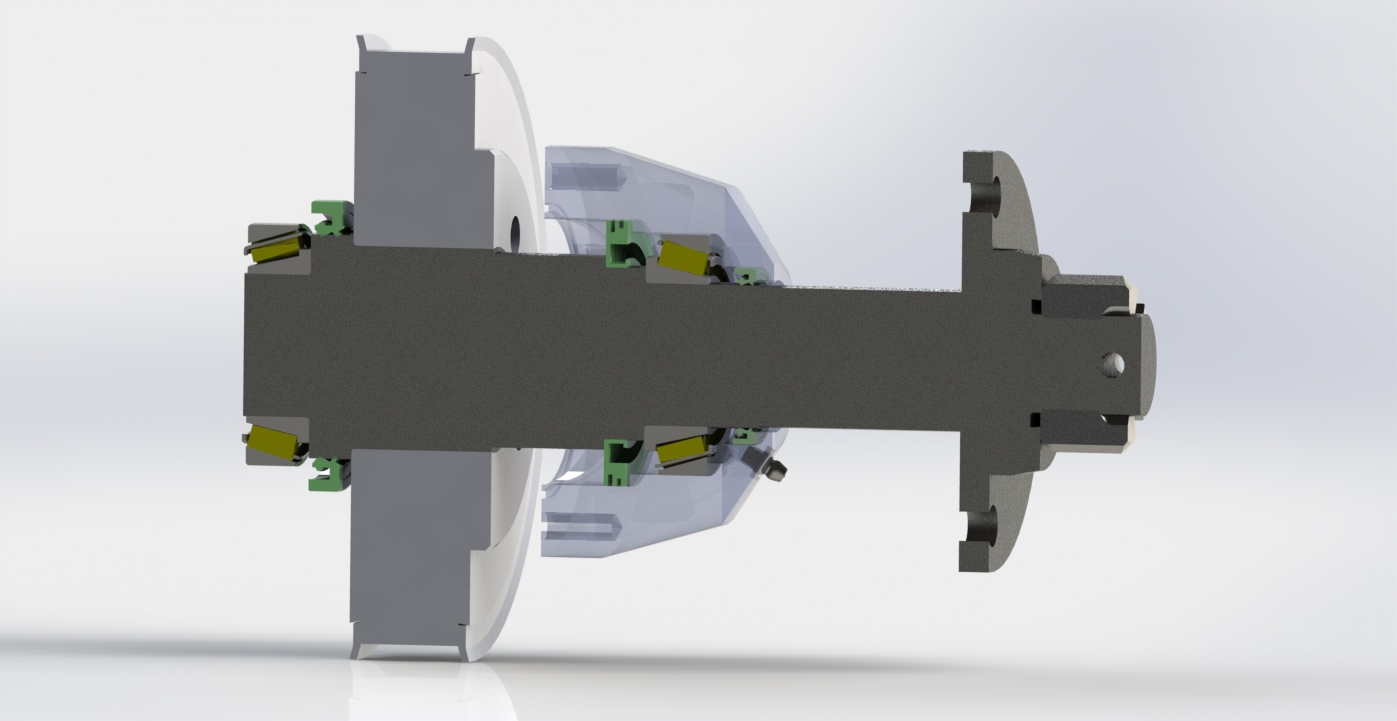
\includegraphics[width=.7\linewidth]{images/wheel_shaft_section.jpg}
	\caption{Section view of wheel shaft assembly.}
	\label{fig:wheel_section}
\end{figure}

\begin{table}[htbp]
	\centering
	\caption{Component details for wheel shaft assembly.}
	\begin{tabular}{| lll |} \hline
		Component & Material & Product Number \\ \hline
		Wheel Shaft & 4340 Steel (Q/T @ 650\degree C) & - \\
		Housing & 6061 Aluminum & - \\
		Rim Mount & 1045 Steel & - \\
		Taper Roller Bearing & - & 32009 X/Q \\
		Large Seal & - & 68x90x10 DL \\
		Medium Seal & - & 2129B \\
		Small Seal & - & 45x55x7 DL \\
		1.25" Castle Nut & Steel & - \\ \hline
	\end{tabular}
	\label{tab:design_spec}
\end{table}


\subsection{Design Constraints and Functional Requirements}
\subsubsection{Wheel Shaft}
The combination of the weight of the vehicle and the forces imposed by the skid steer amounted to large values, thus requiring a strong and durable shaft that experienced minimal flex. Also to consider was the offset imposed by the centered rims on the tires. Clearance between the tires and drive box needed to be large enough to prevent any contact between the two and this in turn increased the overall length of the shaft,and also increasing the large cantilever loading. The shoulders and step diameters on the shaft also needed to match the available sizing of bearings, seals and bushings. It was advised by Penguin ASI that the shafts be made of 4340 steel that is quenched and tempered at 650℃ for availability, machinability and for company standards reasons.

\subsubsection{Wheel Bearings}
The bearings for this application needed to withstand the large axial forces due to the aggressive skid steer motions and still handle the weight of the vehicle. Size was also an important consideration as larger bearings would directly increased the size of other components such as bearing housings.

\subsubsection{Front Bearing Housing}
The front bearing housing had many factors affecting its design. It need to house the taper roller bearings that were mounted onto the shaft. In addition, an o-ring groove needed to be added to meet the sealing requirements and two radial seals needed to be added on each side of the bearing. It also needed to be quick and easy to machine. 

\subsubsection{Rear Bearing Housing}
The rear bearing housing serves the same purpose as the front one. It must support the loads applied as well as retained the bearing and provide adequate sealing by means of an o-ring. It must also accommodate a radial seal for the rear bearing and must be a slim as possible to prevent any contact between its back edge and the body shell of the unit under extreme loading conditions.


\subsubsection{Rim Mount}
The rim mount needed to feature a self centering system for ease of installation. Manufacturability was also an important consideration as splines could be costly, while a taper design is cheap and quick. The component also need to withstand all the imposed forces and be easy to replicate for future units. Using in stock materials was also an added bonus for the client.

\subsubsection{Shaft Seals}
Two different style of seals were needed for the proposed method of assembly and shaft layout. The front-interior seal needed shaft mounted, meaning it would be pressed onto the shaft and would seal against the housing while the two outer ones were pressed into their housings and sealed against the shaft. All seals needed to be economical, durable and standard size for availability reasons. Penguin ASI also recommended using seals covered with a nitrile rubber coating for optimal sealing and to meet company standards.

%\subsection{Functional Requirements}
\subsection{Analysis and Design}
\subsubsection{Wheel Shaft}
First step of the design was to set up the shaft layout. Since the belt design had already been done, the dimensions and style of bushings for the sprockets were already known. A certain width was then set aside for bearing allowance and rim mount location was predetermined to be at the very end of the shaft. The centered rims also required a minimum distance between the drivebox panel and tire. Giving these conditions, a preliminary shaft layout is seen in ***INSERT FIGURE***.

Given the previously mentioned loading conditions and general shaft layout, a Matlab script was created to calculate the reaction forces throughout the shaft and generate moment diagrams. A second Matlab script was created to calculate the minimum shaft diameters based the DE Goodman method using previously calculated moments, material properties and shaft features such as keys, fillets and shoulder sizes.

The results obtained from the Matlab script were unreasonably large, however many machine design books state that the DE Goodman is simply a conservative estimate, therefore further finite element analysis using software was conducted. The static simulation resulted in reduced, but more acceptable diameters. 
~\ref {tab:shaft_calc}

\begin{table}[htbp]
	\centering
	\caption{Summary of forces acting on the wheel shaft.}
	\begin{tabular}{| llll |} \hline
		Name & Variable & Value & Unit \\
		Radial Force at wheel & F\textsubscript{ar} & 7600.00 & N \\
		Tangential Force at wheel & F\textsubscript{at} & 546.80 & N \\
		Radial Force at outside bearing & F\textsubscript{br} & 18950.00 & N \\
		Tangential Force at outside bearing & F\textsubscript{bt} & 2333.00 & N \\
		Radial Force at sprocket & F\textsubscript{cr} & 1470.00 & N \\
		Tangential Force at sprocket & F\textsubscript{ct} & 4007.00 & N \\
		Radial Force at inner bearing & F\textsubscript{dr} & 9900.00 & N \\
		Tangential Force at inner bearing & F\textsubscript{dt} & 2220.00 & N \\
		Skid Force & F\textsubscript{skid} & 2476.00 & N \\
		Moment Skid & M\textsubscript{skid} & 566.00 & N \\
		Moment Weight & M\textsubscript{weight} & 48.00 & N \\ \hline
	\end{tabular}
	\label{tab:shaft_calc}
\end{table}

\begin{figure}[h]\centering
	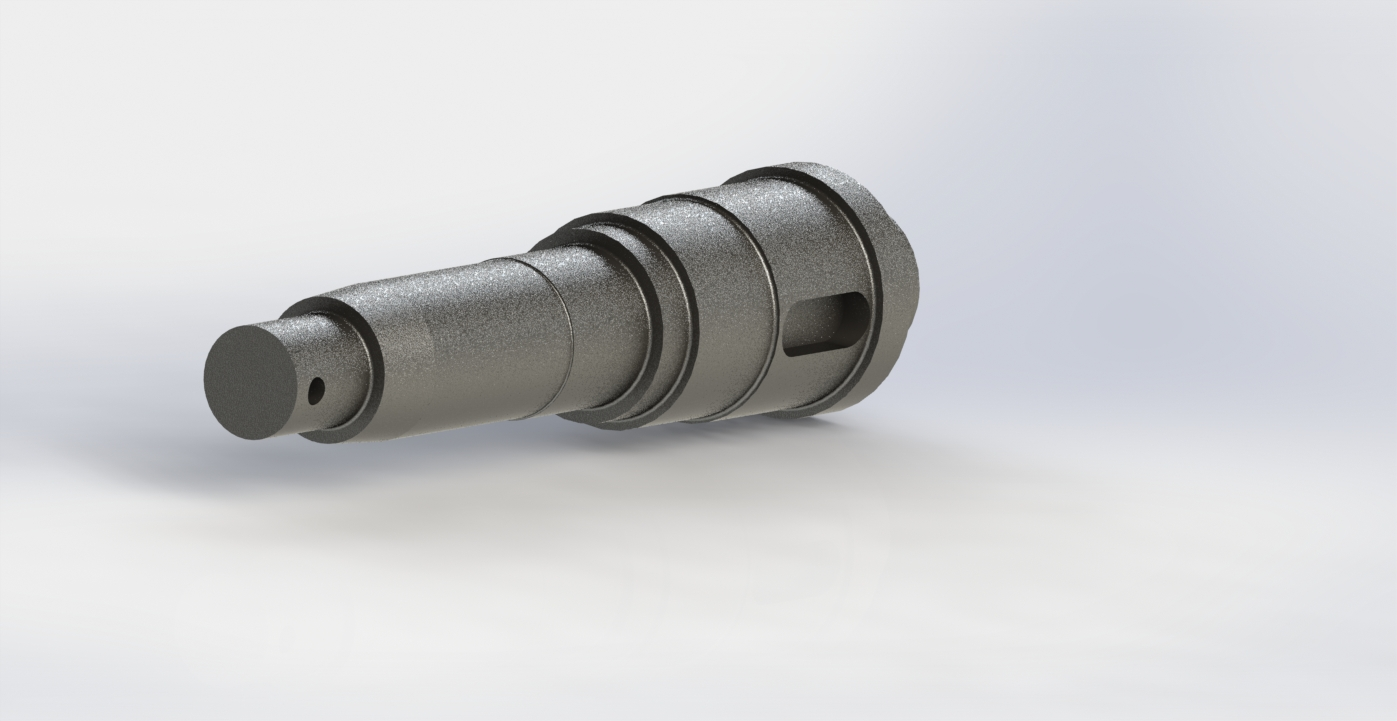
\includegraphics[width=.7\linewidth]{dom/shaft_iso_rndr.jpg}
	\caption{Wheel Shaft}
	\label{fig:wheel_shaft}
\end{figure}

\begin{figure}[h]\centering
	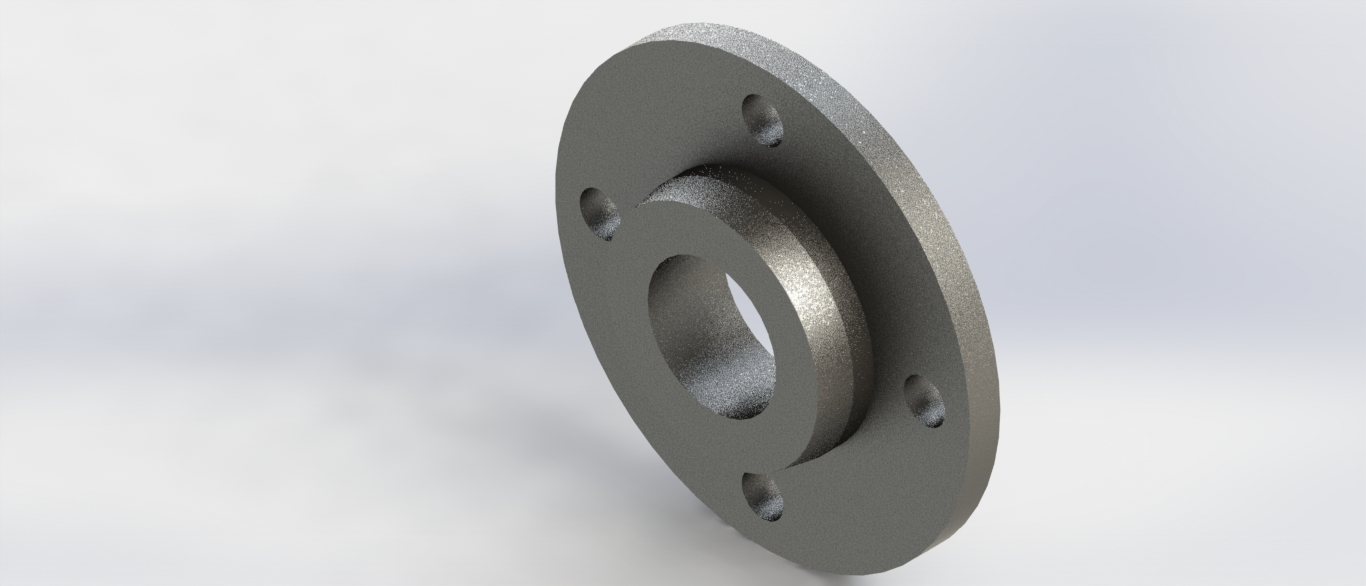
\includegraphics[width=.7\linewidth]{dom/rim_mount_iso_rndr.jpg}
	\caption{Rim Mount}
	\label{fig:rid_mount}
\end{figure}

\subsubsection{Wheel Bearings}
Taper roller bearings were selected for their superior axial loading capabilities while still having decent radial loading ratings when compared to other tradition radial bearings. Size for size, these bearings were still competitive as well. Once bearing type was selected, the bearing selection procedure outlined in the SKF Bearing Manual was followed in order to find the optimal bearing for the task. Based on the reaction forces calculated for the wheel shaft and its diameter, properly sized bearings were selected. A proper assessment also included bearing life calculations and taking into consideration the added axial forces by the taper roller bearings. Since the wheel shaft is essentially a cantilever beam, the bearing sizes were quite large and two separate bearings were required. One on the front and another on the back size. For compatibility, interchangeability and availability reasons, both bearings were selected to be identical even though the rear one doesn't see nearly as much loading.

Please refer to Section ~\ref{ws_bearing} for detailed work on bearing selection. See bearing calculations to Figure ~\ref{bearing_calc} in Appendix for a detailed outline of the SKF bearing selection process.

\subsubsection{Shaft Seals}
Two type of shaft seals were required for the proposed shaft layout. The two outermost seals are housing mounted seals. These are the most common type of radial seals and offered the largest selection. Knowing the shaft dimensions from bearing selection and shaft diameters, all that needed to be selected is which style of shaft seal to chose. A conventional seal with a rubber nitrile coating was recommended by the professionals at Penguin ASI. As for the second type of seal, the selection wasn't so obvious. This second seal was to be a shaft mounted seal, however selection for these proved to be very limited. Only metric sizes were available and there we large variations in diameters. Choosing the closest one to the minimum diameter calculated that would fit between the bearing and sprocket left only one option, however this SKF seal still came with the preferred nitrile rubber coating.

Please refer to the wheel shaft BOM for detailed part numbers of shaft seals.

\subsubsection{Front Bearing Housings}
There were many constraints to the front bearing housing and with the seals selected, and bearing dimensions known, the design of this part was fairly straight forward. The goal to utilize in-stock material also determined that 5 inch, 6061 aluminum would be used. Once the design was complete, a check of bolt and thread strength was conducted as well as an FEA of the component under the loading conditions obtained during the wheel shaft calculations. An o-ring groove was also added to provide adequate sealing for the drivebox.

\begin{figure}[h]\centering
	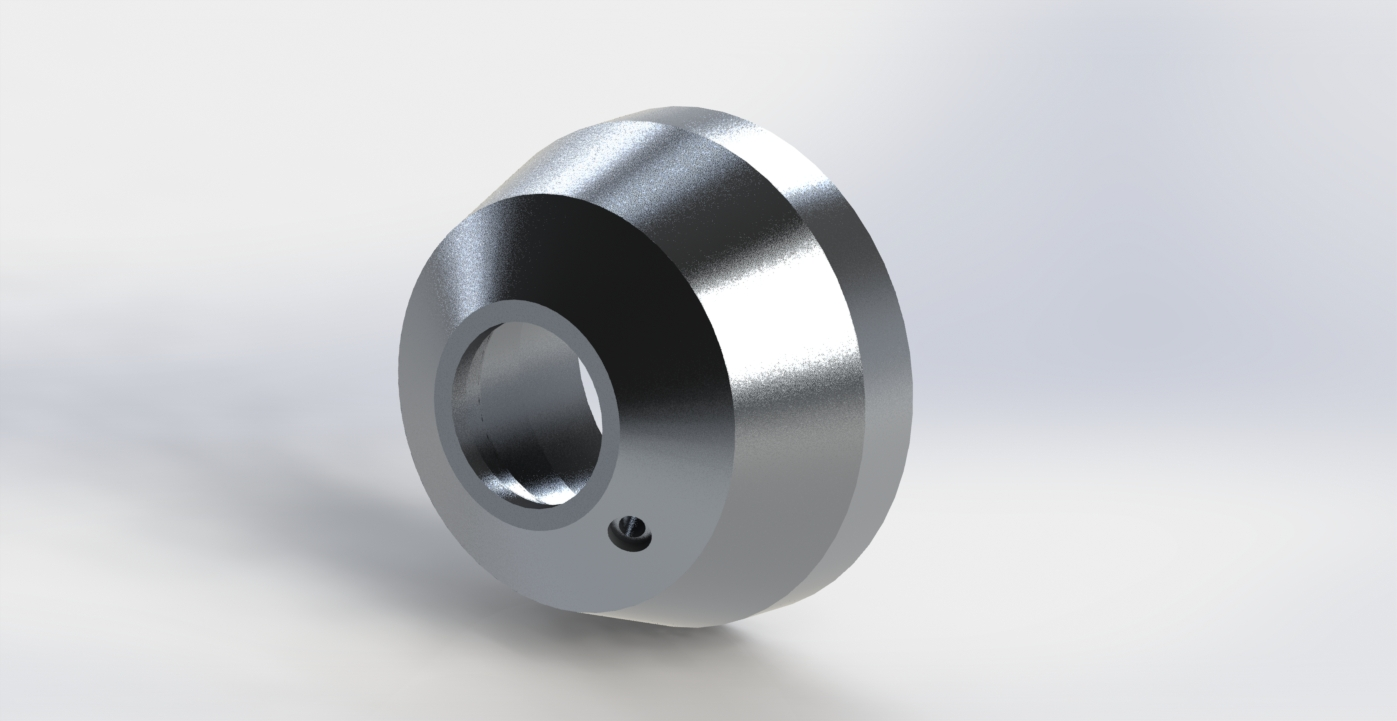
\includegraphics[width=.7\linewidth]{dom/hub_iso_rndr.jpg}
	\caption{Bearing Housing}
	\label{fig:housing}
\end{figure}

Please refer to FEA section of the report for details strength analysis of bearing housing.

\subsubsection{Rear Bearing Housing}
The rear bearing housing was also a straight forward design due to the imposed constraints. For the same reasons as the front bearing housing, 5 inch 6061 round stock was used and a quick verification of bolt and thread strength was conducted. An o-ring groove was also added for sealing purposes.

The final design of this component varied slightly from the initial one. The outer bore was reduced to increase the outer strength of the unit and for better and quick manufacturability. The depth dimensions didn't change, only the outer diameter did. The new design also meant getting rid of the nuts on the back side of the unit as the new design incorporated the thread inside the components, which also simplified the assembly.

Please refer to the FEA Appendix for more details of rear bearing housing design.

\subsubsection{Rim Mount}
The rim mounts from the previous robot were still in good condition and only needed minor modifications for them to meet the requirements of the new design. Modifications included a change to the bolt pattern and boring out the mounting hole onto the shaft. After some calculations, it was determined that a standard taper hole design of 4.18\degree would be strong enough to resist the rotation moments at the wheels and it would mate perfectly with the taper of the wheel shaft for proper mounting. The taper also has the added benefit of self centering, which is crucial for the design of vehicles to prevent unwanted vibrations due to misalignments and poor performance.

\begin{figure}[h]\centering
	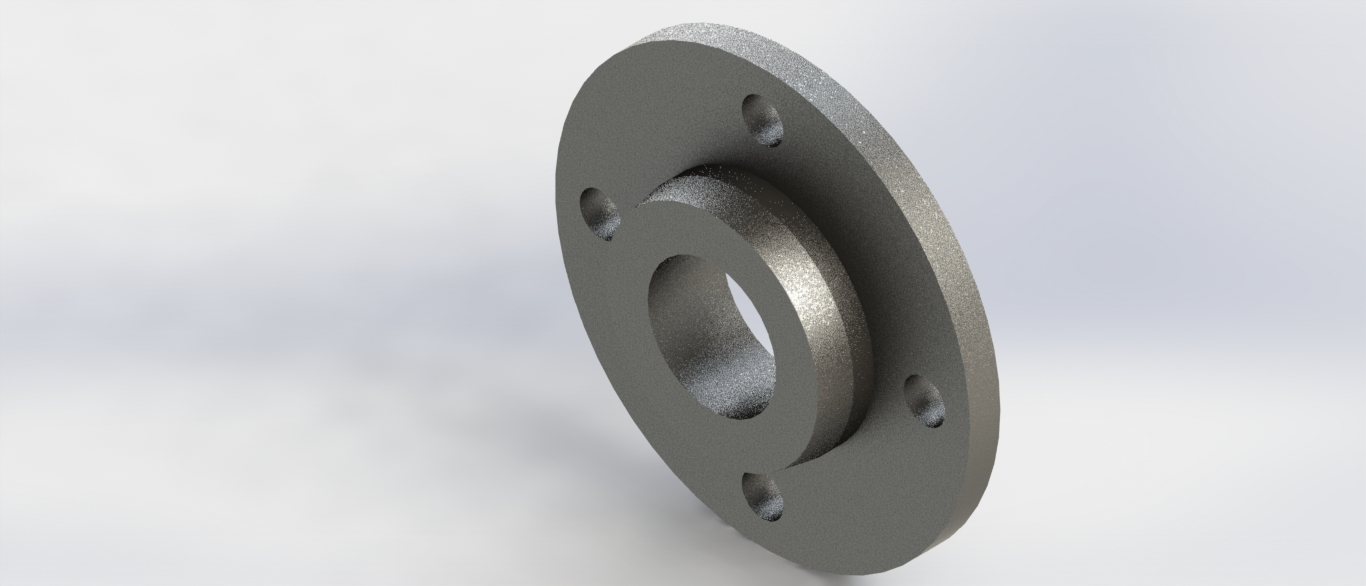
\includegraphics[width=.7\linewidth]{dom/rim_mount_iso_rndr.jpg}
	\caption{Rim Mount}
	\label{fig:rid_mount}
\end{figure}
 

Please refer to Figure ~\ref{taper_calc} for detailed taper strength calculations.
